\section{Double-power density models}
\textbf{Power laws provide excellent descriptions of several astronomical objects;
e.g. a double power law in radius can account for the luminosity density of elliptical galaxies at all radii. Transitioning between large and small radii is described by a model constant, $\gamma$, which is typically set to unity. Dark matter structures has been shown by numerical simulations to be well accounted for wrt. their mass density, by double power laws as well [1].} \\ \\

\centerline{\textbf{Cusp/Core Controversy}} 
The cusp/core problem is relevant when choosing a density profile. In simulations we see a higher degree of halos with central cusps (where $\gamma = -1$), but observations indicate that dwarf galaxies tend to have central cores instead (with $\gamma = 0$). The NFW-profile has a cusp, whereas the Einasto profile has a more flattened central form. The reason for using a HQ density profile instead of a NFW lies in the fact that the HQ has a finite mass, whereas the NFW needs a cut-off. Any physical model for the density must satisfy these conditions: The density profile should be non-negative and finite everywhere in space. It has to decrease smoothly and tend to zero at very large radii. Taking some moments of the mass function, they must be finite, e.g. moments that define the central potential, the total mass, and the effective radius of the system. Finally, the analytical/descriptive functions has to be continuous (no jump discontinuities). Einasto found several groups of descriptive functions where the above criteria are being fulfilled, but the Einasto-profile agrees best with observations. \\

The double power laws described here have the form
\begin{equation}
\rho(r) = \frac{\rho_0}{(\frac{r}{r_s})^{\alpha}(1+(\frac{r}{r_s})^{\gamma})^\frac{\beta-\alpha}{\gamma}}  
\end{equation}
with the transition, $\gamma=1$ for this work.
Most initial structures (see tables of simulations) are set up to follow Hernquist (hereafter HQ) density profiles [22], i.e. \\
\begin{equation} 
\rho_{HQ}(r) = \frac{\rho_0}{(\frac{r}{r_s})(1+\frac{r}{r_s})^3}  
\end{equation}
This is the mass distribution which has been suggested for spherical galaxies by Hernquist in 1990. The normalization constant is given by $\rho_0 = \frac{M}{2\pi}$ , where M is the total mass. For all HQ structures in this work, $M = 1$. Therefore $\rho_0 = \frac{1}{2\pi}$ and the Hernquist profile is simply:
\begin{equation} 
\rho(r) = \frac{1}{2\pi r(1+r)^3}  
\end{equation}
The characteristic scale radius $r_s $ is set to unity throughout. It gives a good description of halo structures. The HQ profile closely resembles the NFW density profile [23], \\
\begin{equation}
\rho_{NFW}(r) = \frac{\rho_0}{(\frac{r}{r_s})(1+\frac{r}{r_s})^2}  
\end{equation}
which has been shown to fit halos in cosmological simulations under a wide range of circumstances. The two mass models differ only for large r, \\
where the NFW profile is diverging towards infinite mass but the HQ profile converges towards a finite mass (Hernquist 1990). 
It turns out that the inner part of structures is insensitive to this difference. It is therefore safe to use either of these two halo profiles if one of them is known to provide a good description of the structure in question. Another density distribution used here is a double power model with $\alpha = 0$ and $\beta = 5$ which takes the form
\begin{equation} 
\rho_{0,5}(r) = \frac{\rho_0}{(1+r)^5}  
\end{equation}
Since the main goal is to determine if an attractor exist in the Jeans parameter space, different density models are needed and starting from a range of different IC's is crucial to determine if they all flow towards any preferred universality for two different types of simulations (here called I and II). In order for this distribution to get a mass of unity, the normalization constant must be $\rho_0 = \frac{3}{\pi}$. The mass of the HQ and NFW profiles are:
\begin{equation}
%\[
    M(r)= 4\pi \rho_0 a^3  
\begin{cases}
    \frac{(\frac{r}{a})^2}{2(1+\frac{r}{a})^2},& \text{HQ} \\
    \ln(1 + \frac{r}{a}) - \frac{\frac{r}{a}}{1 + \frac{r}{a}},& \text{NFW}
\end{cases}
%\]
\end{equation}
Which with normalized total mass and $r_s$ becomes
\begin{equation}
%\[
    M(r)= 2  
\begin{cases}
    \frac{r^2}{2(1+r)^2},& \text{HQ} \\
    \ln(1+r) - \frac{r}{1 + r},& \text{NFW}
\end{cases}
%\]
\end{equation}
And the mass for the $(\alpha,\beta)=(0,5)$ profile is:
\begin{equation} 
M(r) = \int_{0}^{R} \! \rho \cdot 4\pi r^2 \, \mathrm{d}r = 
 \frac{r^3(r+4)}{(r+1)^4}
\end{equation}
With the limit
\begin{equation} 
\lim_{r \to +\infty} M = 1
\end{equation}
Which is thus the total mass of structures D1, DS1 and D2. As their particle number are $N = 10^5$, each particle in these 3 Sims have a mass of $m = \frac{1}{6} \cdot 10^{-5}$. A check is provided that plots the numerically computed density together with the analytical expression for the density profile. The two are in good agreement and this is a good support of the C-codes used.
\begin{figure}[!htbp]
\centering
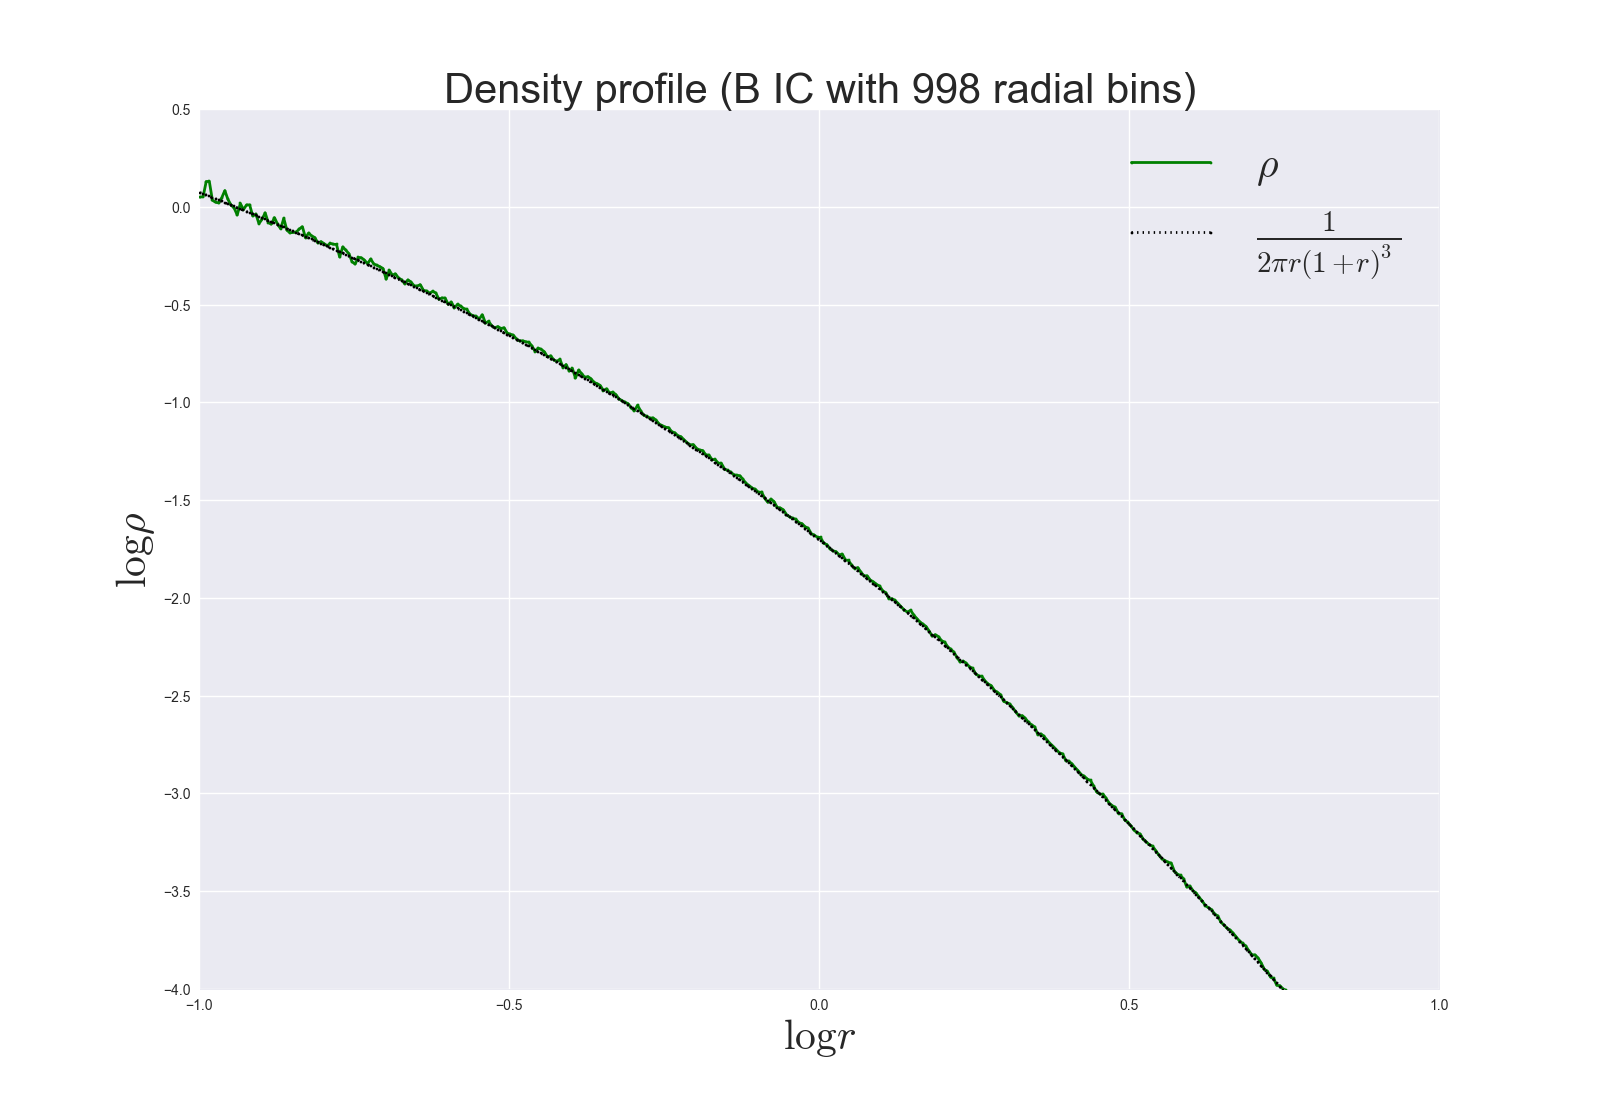
\includegraphics[width=1.0\linewidth]{img/B_Density_fit.png}
\caption{$\rho$ for IC of structure B shown together with analytical expression of HQ profile. The two are in good agreement. Notice the fluctuations at small radii; these can be attributed to Poisson noise. 998 radial bins is used. This structure has a total mass of unity and $N=10^6$ particles, and each particle has a mass of $10^{-6}$ in some arbitrary mass-unit.}
\label{fig:test}
\end{figure}
Since the $\gamma$ profile for all stable structures in dynamical equilibrium have one unique radius where it equals the value -2, hereafter denoted as $r_{-2}$, this radius is a good quantity to normalize radii by in order to better compare different structures. It further introduces a natural unit of length.